\documentclass{beamer}
\usepackage{ctex}
\usepackage{graphicx,booktabs}
\usepackage{tikz}
\usepackage{comment}
\usepackage{multirow}
\usetikzlibrary{arrows,arrows.spaced,arrows.meta,calc,intersections,through,backgrounds,math,angles,shapes}
\usetheme{Boadilla}
\beamersetaveragebackground{black!6}
\def\mathfamilydefault{\rmdefault}
\setbeamersize{text margin left=1.3cm}\setbeamersize{text margin right=1.2cm}
\newcommand\mytitle[1]{\title{#1}\author{王崇宁}\institute[四中]{郑州四中}\logo{
\includegraphics[width=1cm]{cows.jpg}}\maketitle\kaishu\Large}
\newcommand\colorwordsa[1]{\textcolor[rgb]{0,.63,.91}{\heiti #1}}
\newcommand\colorwordsb[1]{\textcolor[rgb]{.75,.53,.21}{\heiti #1}}
\setbeamercolor{mycolor}{fg=black,bg=pink}
\setbeamercolor{myupcol}{fg=white,bg=purple}
\setbeamercolor{mylowcol}{fg=black,bg=pink}
\newcommand\beamercolortextbox[1]{\settowidth\lengtha{#1}\hspace{.5em}\raisebox{-.6ex}{\begin{beamercolorbox}[rounded=true,shadow=true,wd=\lengtha,colsep*=-.4ex]{mycolor}#1\end{beamercolorbox}}}
\newcommand\beamercolorlinebox[1]{\settowidth\lengtha{#1}\centerline{\begin{beamercolorbox}[rounded=true,shadow=true,wd=\lengtha]{mycolor}#1\end{beamercolorbox}}}\newlength\lengtha
\newcommand\threesides{\begin{picture}(14,12)\put(0,0){\qbezier(0,0)(0,8)(7,12)\qbezier(7,12)(14,8)(14,0)\qbezier(14,0)(7,-4)(0,0)}\end{picture}}


\def\displaygray{\setbeamercovered{transparent}}
\newcommand*\circled[1]{\hspace{1pt}\tikz[baseline=(char.base)]\node[very thin,shape=circle,draw,inner sep=.5pt,minimum size=2pt](char){#1};\hspace{1pt}}%



\newcommand\Dd{\displaystyle}\newcommand{\Tt}{\textstyle}\newcommand{\Ss}{\scriptstyle}\newcommand{\Sss}{\scriptscriptstyle}%

\setlength\mathsurround{0.5ex}%文本公式前后留下空白
\makeatletter
\renewcommand\normalsize{\@setfontsize\normalsize\@xpt\@xiipt\abovedisplayskip8\p@\@plus3\p@\@minus5\p@\abovedisplayshortskip\z@\@plus3\p@\belowdisplayshortskip5\p@\@plus3\p@\@minus7\p@\belowdisplayskip\abovedisplayskip\let\@listi\@listI}%行间公式上下
\@addtoreset{equation}{section}
\renewcommand\theequation{\oldstylenums{\thesection}.\oldstylenums{\arabic{equation}}}%公式按章节编号
\makeatother
%\setlength\mathsurround{0.ex}%数学模式与文本模式混排时留出的间距

\newcommand\an[1][a]{\ensuremath{\{#1_n\}}}%sequence
\newcommand\ud{\mathrm{d}}
\newcommand{\ue}{\mathrm{e}}%正体字母
\newcommand\triabc{\ensuremath{\triangle ABC}}%三角形ABC
\newcommand\cnm[2][n]{\ensuremath{\textrm{C}^{#2}_{#1}}}%组合数
%数学题目编辑
\newcommand\lines[1][1.2]{\,\underline{\mbox{\hspace{#1cm}}}\,}% 填空题的横线
\newcommand\brackets[1][2]{\nolinebreak\hfill\mbox{~(\hspace{#1em})}\\}% 选择题的括号
%扩展命令
\newcommand\qqquad{\qquad\quad}
\def\aside#1{\marginpar{\footnotesize #1}}
%自动编号之最简
\newcommand\numa{\refstepcounter{numi}\thenumi}\newcounter{numi}
\newcommand\numb{\refstepcounter{numii}\thenumii}\newcounter{numii}
\newcommand\numc{\refstepcounter{numiii}\thenumiii}\newcounter{numiii}
\newcommand\numaa{\refstepcounter{numai}\thenumai}\newcounter{numai}[numi]

\newcommand{\question}[1][]{\par\vspace{1ex}\noindent\refstepcounter{numberi}\textbf{\thenumberi.}\ensuremath{#1}}\newcounter{numberi}[subsection]% 每道小题自动编号
\newcommand\quson{\\ \hspace*{1em}\refstepcounter{numberii}\thenumberii)~}\newcounter{numberii}[numberi]% 每道小题自动编号
\newcommand\choice[5][4]{\vspace*{-1em}\begin{tasks}(#1)\task$#2$\task$#3$\task$#4$\task$#5$\end{tasks}\vspace*{-1.2em}}%选择题排版之数学模式
\newcommand\choicex[5][4]{\vspace*{-1em}\begin{tasks}(#1)\task#2\task#3\task#4\task#5\end{tasks}\vspace*{-1.2em}}%选择题排版之yysg模式
\newcommand\tbs[1][]{\texttt{\char92#1}}

\newcommand\set[1]{\lbrace\ensuremath{#1}\rbrace}
\newcommand\setx[1]{\{#1\}}

\newcommand\mybf[1]{{\bm#1}}
\def\bfR{\mybf R}
\def\bfN{\mybf N}
\def\bfZ{\mybf Z}
\def\bfQ{\mybf Q}
\def\bfC{\mybf C}
\def\bfZp{\mybf Z^+}

\newcommand\myvec[1]{\bm#1}
\def\veca{\myvec a}
\def\vecb{\myvec b}
\def\vecc{\myvec c}
\def\vecd{\myvec d}
\def\vece{\myvec e}
\def\vecf{\myvec f}
\def\vecs{\myvec e}
\def\vecp{\myvec p}
\def\vecq{\myvec q}
\def\veci{\myvec i}
\def\vecj{\myvec j}
\def\vecei{\myvec{e_1}}
\def\veceii{\myvec{e_2}}
\def\veczero{\myvec 0}
\newcommand\lvec[1]{\overrightarrow{#1}}





\begin{document}
\mytitle{有理数的乘方}
\makeatletter
\renewcommand\normalsize{\@setfontsize\normalsize\@xpt\@xiipt\abovedisplayskip8\p@\@plus3\p@\@minus5\p@\abovedisplayshortskip\z@\@plus3\p@\belowdisplayshortskip5\p@\@plus3\p@\@minus7\p@\belowdisplayskip\abovedisplayskip\let\@listi\@listI}%行间公式上下
\makeatother
\begin{frame}{本杰明$\cdot$富兰克林的遗嘱}\Large\songti
  现将一千英镑赠与波士顿的居民.
  如果他们接受这一千英镑,
  那么这笔钱应该托付给一些德高望重的人士,
  由他们负责把这笔钱以\underline{每年百分之五的利率}借给年轻的手工业者们去生息.
  \underline{$100$年后这笔钱将增至$131\,000$英镑.}
\end{frame}


\begin{comment}
\begin{frame}
  $1$年后$x=1000\times1.05$\\ \pause

  $2$年后$x=1000\times1.05^2$\\\pause%这个小2表示有二个1.05相乘

  $3$年后$x=1000\times1.05^3$\\\pause%这个小3表示有三个1.05相乘

  \dots\\

  $100$年后$x=1000\times1.05^{100}$\\\pause%这个100表示有100个1.05相乘
\end{frame}

\begin{frame}
  $a\times a=a^2$ \pause

  $a\times a\times a=$ $a^3$\pause

  $a\times a\times a\times a\times a=$ \pause $a^5$ \pause

  $\underbrace{a\times a\times a\times\cdots\times a}_{n\text{个}a}=$\pause$a^n$  \pause
\end{frame}
\end{comment}


\begin{frame}{学习目标}
  \begin{block}{}
    \begin{itemize}
      \item 能够说出乘方的定义.\\\pause
      \item 能够把特定问题中的算式用乘方表示出来, 并正确计算简单的乘方.\\
    \end{itemize}
  \end{block}
\end{frame}


\begin{frame}
  \begin{block}{思考}
    $n$个相同的数相加定义了\colorwordsb{乘法}\par\pause
    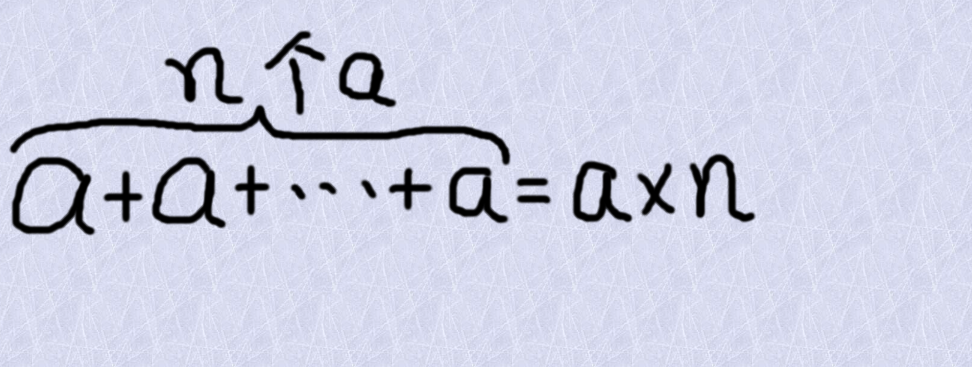
\includegraphics[width=2.5in]{times01.png}\par
  \end{block}
\end{frame}
\begin{frame}
  \begin{block}{思考}
    $n$个相同的数相加定义了\colorwordsb{乘法}\par
    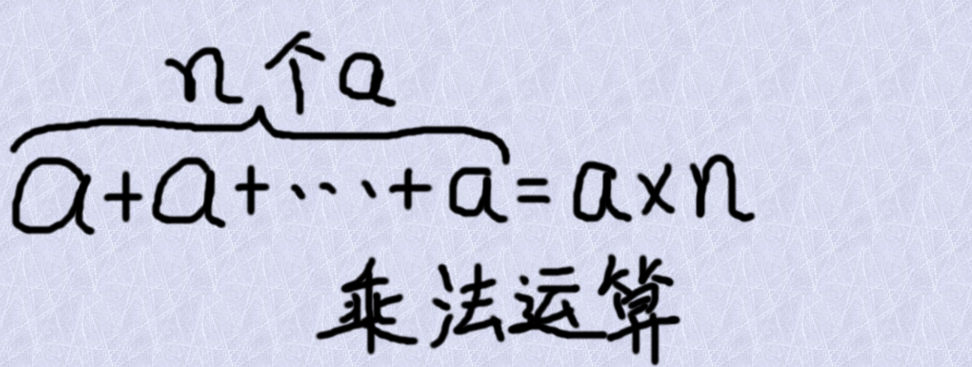
\includegraphics[width=2.5in]{times02.png}\par
  \end{block}
\end{frame}
\begin{frame}
  \begin{block}{思考}
    $n$个相同的数相加定义了\colorwordsb{乘法}\par
    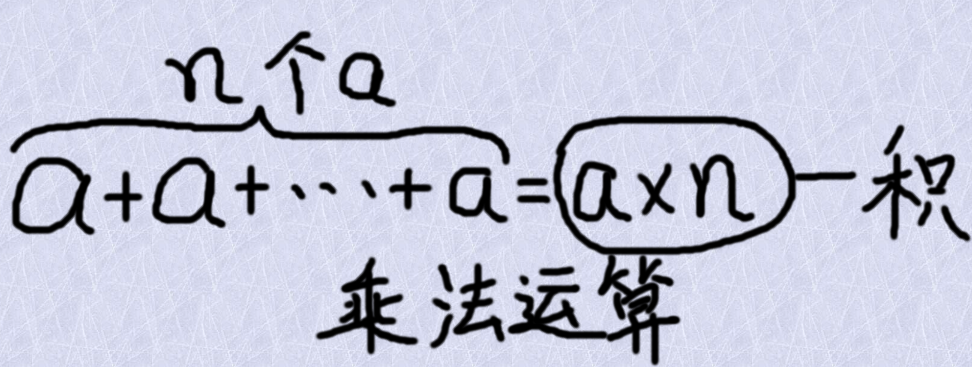
\includegraphics[width=2.5in]{times03.png}\par
  \end{block}
\end{frame}
\begin{frame}
  \begin{block}{思考}
    $n$个相同的数相加定义了\colorwordsb{乘法}\par
    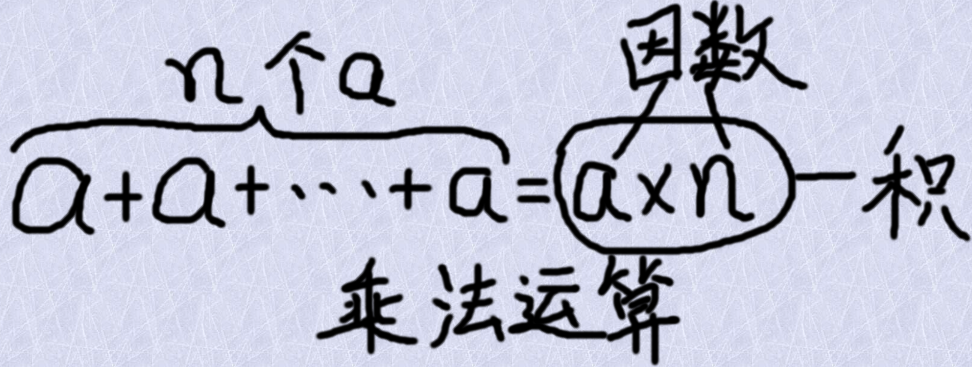
\includegraphics[width=2.5in]{times04.png}\par
  \end{block}
\end{frame}
\begin{frame}
  \begin{block}{思考}
    $n$个相同的数相加定义了\colorwordsb{乘法}\par
    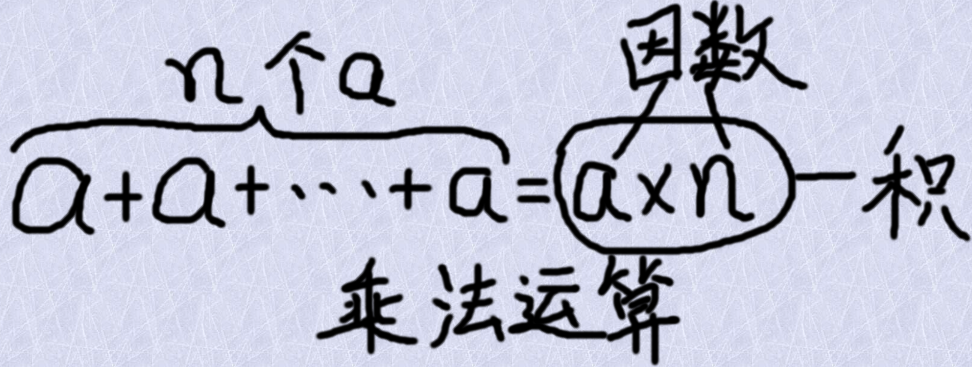
\includegraphics[width=2.5in]{times04.png}\par\pause
    $n$个相同的数相乘可定义\colorwordsb{乘方} \\\vspace*{-2em}
    $$\underbrace{a\times a\times\cdots\times a}_{n\text{个}a}=a^n$$  
  \end{block}
\end{frame}


\begin{frame}{定义}
  \begin{block}{}
    为简便, 一般地, $n$个相同的因数$a$相乘, 记作$a^n$, 即
      $$\underbrace{a\times a\times\cdots\times a}_{n\text{个}a}=a^n$$  
    这种求$n$个相同因数$a$的积的运算叫做\colorwordsa{乘方}, 乘方的结果叫做\colorwordsa{幂}, $a$叫做底数, $n$叫做指数, 
$a^n$读作\colorwordsb{$a$的$n$次幂}(或\colorwordsb{$a$的$n$次方}).
  \end{block}
\end{frame}


\begin{frame}{根据定义计算}\LARGE
  \begin{exampleblock}{例1.计算:}
    $(1)\ 5^3$ \pause $=5\times5\times5$ \pause    

     $(2) (-3)^4$ \pause $=(-3)\times(-3)\times(-3)\times(-3)$ \pause\\
     \hspace*{4.3em}$=+(3\times3\times3\times3)=81$\\
  \end{exampleblock}
\end{frame}

\begin{frame}{根据定义计算}
  \begin{block}{练习1}
    (1)$(-1.5)^1$ ;\quad (2)${(\frac32)}^2$ ;\\ \pause 
    (3)$(-0.3)^3$ ;\quad (4)$-3^4$.
  \end{block}
\end{frame}

\begin{frame}\Huge
  $$(-3)^4~\text{和}~-3^4~\text{的区别在哪里?}$$
\end{frame}

\newlength\laa\newlength\lbb
\settowidth\laa{(-3)x(-3)x(-3)x(-3)}\settowidth\lbb{4个3相乘再取相反数}
\def\tia{\makebox[\laa]{\ }}\def\tib{\makebox[\lbb]{\ }}
\begin{frame}\begin{table}[htbp]\centering\begin{tabular}{l|c|c}
      \toprule      \ & $(-3)^4$ & $-3^4$ \\
      \hline\hline  写法 & \tia & \tib \\
      \hline        读法 & \tia & \tib \\
      \hline        \multirow{2}{*}{意义} &\tia &\tib \\
                    &\tia & \tib\\
      \hline       结果 & \tia &  \\
\bottomrule\end{tabular}\end{table}\end{frame}
\begin{frame}\begin{table}[htbp]\centering\begin{tabular}{l|c|c}
      \toprule      \ & $(-3)^4$ & $-3^4$ \\
      \hline\hline  写法 & 有括号 & \tib \\
      \hline        读法 &\tia  & \\
      \hline        \multirow{2}{*}{意义} &  &  \\
                    & & \\
      \hline       结果 & &  \\
\bottomrule\end{tabular}\end{table}\end{frame}
\begin{frame}\begin{table}[htbp]\centering\begin{tabular}{l|c|c}
      \toprule      \ & $(-3)^4$ & $-3^4$ \\
      \hline\hline  写法 & 有括号 & 无括号 \\
      \hline        读法 & \tia & \tib \\
      \hline        \multirow{2}{*}{意义} & &  \\
                    & &\\
      \hline       结果 & &  \\
\bottomrule\end{tabular}\end{table}\end{frame}
\begin{frame}\begin{table}[htbp]\centering\begin{tabular}{l|c|c}
      \toprule      \ & $(-3)^4$ & $-3^4$ \\
      \hline\hline  写法 & 有括号 & 无括号 \\
      \hline        读法 & 负3的4次方 & \tib \\
      \hline        \multirow{2}{*}{意义} & \tia &  \\
                    & & \\
      \hline       结果 & &  \\
\bottomrule\end{tabular}\end{table}\end{frame}
\begin{frame}\begin{table}[htbp]\centering\begin{tabular}{l|c|c}
      \toprule      \ & $(-3)^4$ & $-3^4$ \\
      \hline\hline  写法 & 有括号 & 无括号 \\
      \hline        读法 & 负3的4次方 & 3的4次方的相反数 \\
      \hline        \multirow{2}{*}{意义} & \tia&\tib \\
                    & & \\
      \hline       结果 &  &  \\
\bottomrule\end{tabular}\end{table}\end{frame}
\begin{frame}\begin{table}[htbp]\centering\begin{tabular}{l|c|c}
      \toprule      \ & $(-3)^4$ & $-3^4$ \\
      \hline\hline  写法 & 有括号 & 无括号 \\
      \hline        读法 & 负3的4次方 &3的4次方的相反数  \\
      \hline        \multirow{2}{*}{意义} & 4个$(-3)$相乘 &  \\
                    & & \\
      \hline       结果 &\tia  & \tib \\
\bottomrule\end{tabular}\end{table}\end{frame}
\begin{frame}\begin{table}[htbp]\centering\begin{tabular}{l|c|c}
      \toprule      \ & $(-3)^4$ & $-3^4$ \\
      \hline\hline  写法 & 有括号 & 无括号 \\
      \hline        读法 & 负3的4次方 & 3的4次方的相反数 \\
      \hline        \multirow{2}{*}{意义} & 4个$(-3)$相乘 & \\
                    &(-3)x(-3)x(-3)x(-3) &\\
      \hline       结果 & \tia &\tib  \\
\bottomrule\end{tabular}\end{table}\end{frame}
\begin{frame}\begin{table}[htbp]\centering\begin{tabular}{l|c|c}
      \toprule      \ & $(-3)^4$ & $-3^4$ \\
      \hline\hline  写法 & 有括号 & 无括号 \\
      \hline        读法 & 负3的4次方 &  3的4次方的相反数\\
      \hline        \multirow{2}{*}{意义} & 4个$(-3)$相乘 & 4个3相乘再取相反数 \\
                    &(-3)x(-3)x(-3)x(-3) & \\
      \hline       结果 & \tia & \tib \\
\bottomrule\end{tabular}\end{table}\end{frame}
\begin{frame}\begin{table}[htbp]\centering\begin{tabular}{l|c|c}
      \toprule      \ & $(-3)^4$ & $-3^4$ \\
      \hline\hline  写法 & 有括号 & 无括号 \\
      \hline        读法 & 负3的4次方 & 3的4次方的相反数 \\
      \hline        \multirow{2}{*}{意义} & 4个$(-3)$相乘 & 4个3相乘再取相反数 \\
                    &(-3)x(-3)x(-3)x(-3) & -(3x3x3x3)\\
      \hline       结果 & \tia &\tib \\
\bottomrule\end{tabular}\end{table}\end{frame}
\begin{frame}\begin{table}[htbp]\centering\begin{tabular}{l|c|c}
      \toprule      \ & $(-3)^4$ & $-3^4$ \\
      \hline\hline  写法 & 有括号 & 无括号 \\
      \hline        读法 & 负3的4次方 & 3的4次方的相反数 \\
      \hline        \multirow{2}{*}{意义} & 4个$(-3)$相乘 & 4个3相乘再取相反数 \\
                    &(-3)x(-3)x(-3)x(-3) & -(3x3x3x3)\\
      \hline       结果 & 81 & -81 \\
\bottomrule\end{tabular}\end{table}\end{frame}



\begin{frame}{练习}
  \begin{block}{练习2.}
    $(1)\ (-2)^2$; \qquad $(2)\ -2^4$; \qquad $(3)\ -(-2)^4$.
  \end{block}
\end{frame}
\begin{frame}{练习}
  \begin{block}{练习3.}
    $(1)\ \Dd(-\frac34)^2$; \qquad $(2)\ \Dd-\frac{3^2}4$; \qquad $(3)\ \Dd-(\frac34)^2$.  
  \end{block}
\end{frame}




\begin{comment}
\begin{frame}
我希望拿出其中的$100\,000$英镑建造一所公共建筑物,其余的$31\,000$英镑继续借出去生息.

第二个$100$年,这笔钱将增加到$4\,061\,000$,其中的$1\,061\,000$英镑继续由波士顿的居民支配,而剩下的$3\,000\,000$英镑留给马萨诸赛州的公众来管理.再往后的事情,我可不擅作主张了.
\end{frame}
\end{comment}


\begin{frame}{这节课你学到了什么?}
  \begin{exampleblock}{问题:}
    你到今天为止都学过哪些运算? 乘方是我们学习的第几种运算?
  \end{exampleblock}\pause
  \begin{block}{}
    \begin{table}[htbp]\large
      \centering
      \begin{tabular}{c|c|c|c|c|c}
        \hline
        \ & 第一种 & 第二种 & 第三种 & 第四种 & 第五种\\
        \hline
        运算 & 加法 & 减法 & 乘法 & 除法 & 乘方\\
        \hline
        优先级 & \multicolumn{2}{c}{第一级} & \multicolumn{2}{c}{第二级} & 第三级\\
        \hline
      \end{tabular}
    \end{table}
  \end{block}
\end{frame}

\begin{frame}
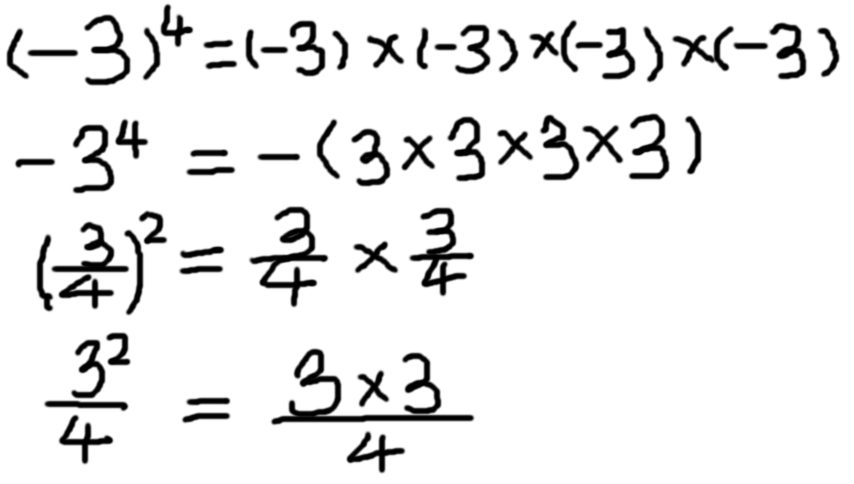
\includegraphics[width=3in]{_34_34.png}
\end{frame}


begin{frame}\begin{table}[htbp]\centering\begin{tabular}{l|c|c}
      \toprule      \ & $(-3)^4$ & $-3^4$ \\
      \hline\hline  写法 & \tia & \tib \\
      \hline        读法 & \tia & \tib \\
      \hline        \multirow{2}{*}{意义} &\tia &\tib \\
                    &\tia & \tib\\
      \hline       结果 & \tia &  \\
\bottomrule\end{tabular}\end{table}\end{frame}
\begin{frame}\begin{table}[htbp]\centering\begin{tabular}{l|c|c}
      \toprule      \ & $(-3)^4$ & $-3^4$ \\
      \hline\hline  写法 & 有括号 & \tib \\
      \hline        读法 &\tia  & \\
      \hline        \multirow{2}{*}{意义} &  &  \\
                    & & \\
      \hline       结果 & &  \\
\bottomrule\end{tabular}\end{table}\end{frame}
\begin{frame}\begin{table}[htbp]\centering\begin{tabular}{l|c|c}
      \toprule      \ & $(-3)^4$ & $-3^4$ \\
      \hline\hline  写法 & 有括号 & 无括号 \\
      \hline        读法 & \tia & \tib \\
      \hline        \multirow{2}{*}{意义} & &  \\
                    & &\\
      \hline       结果 & &  \\
\bottomrule\end{tabular}\end{table}\end{frame}
\begin{frame}\begin{table}[htbp]\centering\begin{tabular}{l|c|c}
      \toprule      \ & $(-3)^4$ & $-3^4$ \\
      \hline\hline  写法 & 有括号 & 无括号 \\
      \hline        读法 & 负3的4次方 & \tib \\
      \hline        \multirow{2}{*}{意义} & \tia &  \\
                    & & \\
      \hline       结果 & &  \\
\bottomrule\end{tabular}\end{table}\end{frame}
\begin{frame}\begin{table}[htbp]\centering\begin{tabular}{l|c|c}
      \toprule      \ & $(-3)^4$ & $-3^4$ \\
      \hline\hline  写法 & 有括号 & 无括号 \\
      \hline        读法 & 负3的4次方 & 3的4次方的相反数 \\
      \hline        \multirow{2}{*}{意义} & \tia&\tib \\
                    & & \\
      \hline       结果 &  &  \\
\bottomrule\end{tabular}\end{table}\end{frame}
\begin{frame}\begin{table}[htbp]\centering\begin{tabular}{l|c|c}
      \toprule      \ & $(-3)^4$ & $-3^4$ \\
      \hline\hline  写法 & 有括号 & 无括号 \\
      \hline        读法 & 负3的4次方 &3的4次方的相反数  \\
      \hline        \multirow{2}{*}{意义} & 4个$(-3)$相乘 &  \\
                    & & \\
      \hline       结果 &\tia  & \tib \\
\bottomrule\end{tabular}\end{table}\end{frame}
\begin{frame}\begin{table}[htbp]\centering\begin{tabular}{l|c|c}
      \toprule      \ & $(-3)^4$ & $-3^4$ \\
      \hline\hline  写法 & 有括号 & 无括号 \\
      \hline        读法 & 负3的4次方 & 3的4次方的相反数 \\
      \hline        \multirow{2}{*}{意义} & 4个$(-3)$相乘 & \\
                    &(-3)x(-3)x(-3)x(-3) &\\
      \hline       结果 & \tia &\tib  \\
\bottomrule\end{tabular}\end{table}\end{frame}
\begin{frame}\begin{table}[htbp]\centering\begin{tabular}{l|c|c}
      \toprule      \ & $(-3)^4$ & $-3^4$ \\
      \hline\hline  写法 & 有括号 & 无括号 \\
      \hline        读法 & 负3的4次方 &  3的4次方的相反数\\
      \hline        \multirow{2}{*}{意义} & 4个$(-3)$相乘 & 4个3相乘再取相反数 \\
                    &(-3)x(-3)x(-3)x(-3) & \\
      \hline       结果 & \tia & \tib \\
\bottomrule\end{tabular}\end{table}\end{frame}
\begin{frame}\begin{table}[htbp]\centering\begin{tabular}{l|c|c}
      \toprule      \ & $(-3)^4$ & $-3^4$ \\
      \hline\hline  写法 & 有括号 & 无括号 \\
      \hline        读法 & 负3的4次方 & 3的4次方的相反数 \\
      \hline        \multirow{2}{*}{意义} & 4个$(-3)$相乘 & 4个3相乘再取相反数 \\
                    &(-3)x(-3)x(-3)x(-3) & -(3x3x3x3)\\
      \hline       结果 & \tia &\tib \\
\bottomrule\end{tabular}\end{table}\end{frame}
\begin{frame}\begin{table}[htbp]\centering\begin{tabular}{l|c|c}
      \toprule      \ & $(-3)^4$ & $-3^4$ \\
      \hline\hline  写法 & 有括号 & 无括号 \\
      \hline        读法 & 负3的4次方 & 3的4次方的相反数 \\
      \hline        \multirow{2}{*}{意义} & 4个$(-3)$相乘 & 4个3相乘再取相反数 \\
                    &(-3)x(-3)x(-3)x(-3) & -(3x3x3x3)\\
      \hline       结果 & 81 & -81 \\
\bottomrule\end{tabular}\end{table}\end{frame}


\def\calcpng#1{
\begin{frame}
\hspace*{-2.1cm}\includegraphics[width=5in]{#1}
\end{frame}
}
\calcpng{calc1.png}\calcpng{calc2.png}\calcpng{calc3.png}\calcpng{calc4.png}

\begin{frame}{乘方的世界你还不懂}
  \begin{exampleblock}{}
    \begin{itemize}
      \item 虽然$1.05$是一个很小的数, 但是经过很多次的累乘之后, 它的大小超乎你的想象.

      \item 同样地, 你每一份努力看起来都不那么重要, 但是, 这些努力一点一点地累积起来, 你所能够达到的境界也会超乎你的想象. 
    \end{itemize}
  \end{exampleblock}
\end{frame}

\begin{frame}
  \begin{block}{作业}
    校本作业\ 有理数的乘方(一)
  \end{block}
\end{frame}

\begin{comment}
\begin{frame}
  \begin{block}{小结}
    \begin{enumerate}
      \item 乘方的定义\\
      \item 分数和负数的乘方怎样表示?\\
      \item $(-1)^n$如何计算\\
      \item 一个有理数的平方总是非负的\\
      \item (体会)乘方运算随指数增长变化是极大的\\
    \end{enumerate}
  \end{block}
\end{frame}
\end{comment}

\begin{frame}{拔高训练}\large
  1.一个草履虫平均每经过$27$小时就会分裂成两个.假如以这些方式衍生的草履虫都能存活下来, $27$天之后, 这个草履虫及其后代共有多少个? (用$x^y$表示出来即可.)

  2.计算:(1)$-1.5^2$\qquad (2)$\Dd -\frac{(-2)^4}{4}$ \qquad (3)$\Dd -{(-1\frac12)}^3$

\end{frame}
\end{document}
